\documentclass[dvips,landscape]{foils}
\usepackage{graphicx,psfrag}
\usepackage{graphics}
\usepackage{amsmath}
\usepackage{amsthm}
\usepackage{amsfonts}
\input defs.tex
\raggedright
\special{! TeXDict begin /landplus90{true}store end }
\renewcommand{\oursection}[1]{
\foilhead[-1.0cm]{#1}
}

\title{The Study of 1-D Chaotic Maps}
\author{Tzu-Chen Liang}
\MyLogo{Tzu-Chen Liang, Stanford University}
\date{\today}
\newtheorem{definition}{Definition}
\newtheorem{example}{Example}

\begin{document}
%\setlength{\parskip}{0cm}
\maketitle


%%%%%%%%%%%%%%%%%%%%%%%%%%%%%%%%%%%%%%%%%%%%%%%%%%%%%%%%%%%%%%%%%%%%%%%%%%
\newpage
\oursection{Logistic Map}
\begin{eqnarray*}
 x^{k+1} = cx^k(1-x^k)
\end{eqnarray*}
$c=4$ in all our simulations.
\begin{tabular}{rl}%\setlength{\tabcolsep}{-30mm}
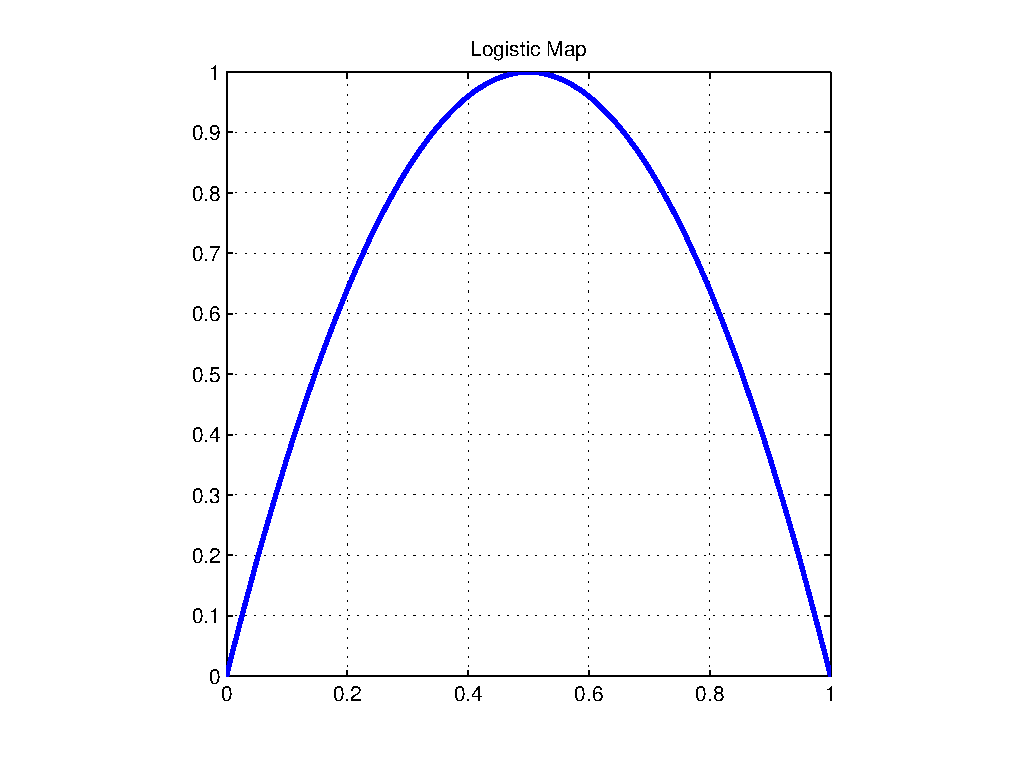
\includegraphics[width=0.44\textwidth,trim=1cm 1cm 0cm 0cm]{logisticmap}&
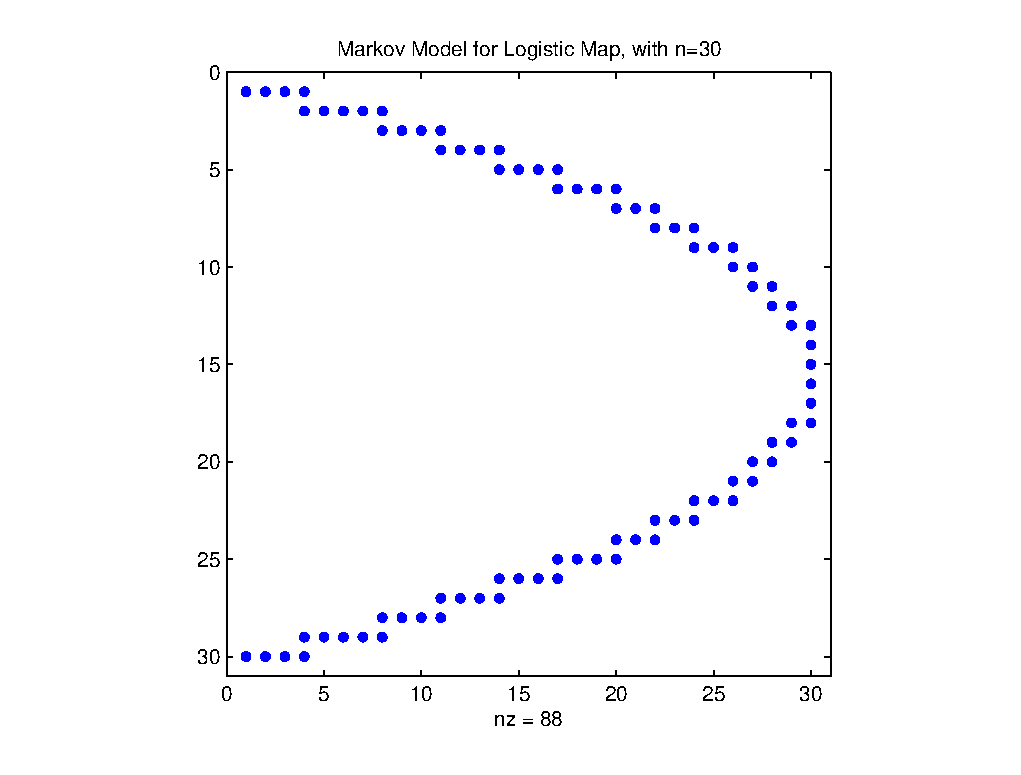
\includegraphics[width=0.44\textwidth,trim=1cm 1cm 0cm 0cm]{logisticmapA}
\end{tabular}
We run simulations with $n$ up to $1e7$. 

%%%%%%%%%%%%%%%%%%%%%%%%%%%%%%%%%%%%%%%%%%%%%%%%%%%%%%%%%%%%%%%%%%%%%%%%%%
\newpage
Cutoffs are observed both in simulations of $A$ and $A^T$. 
\begin{tabular}{rl}%\setlength{\tabcolsep}{-30mm}
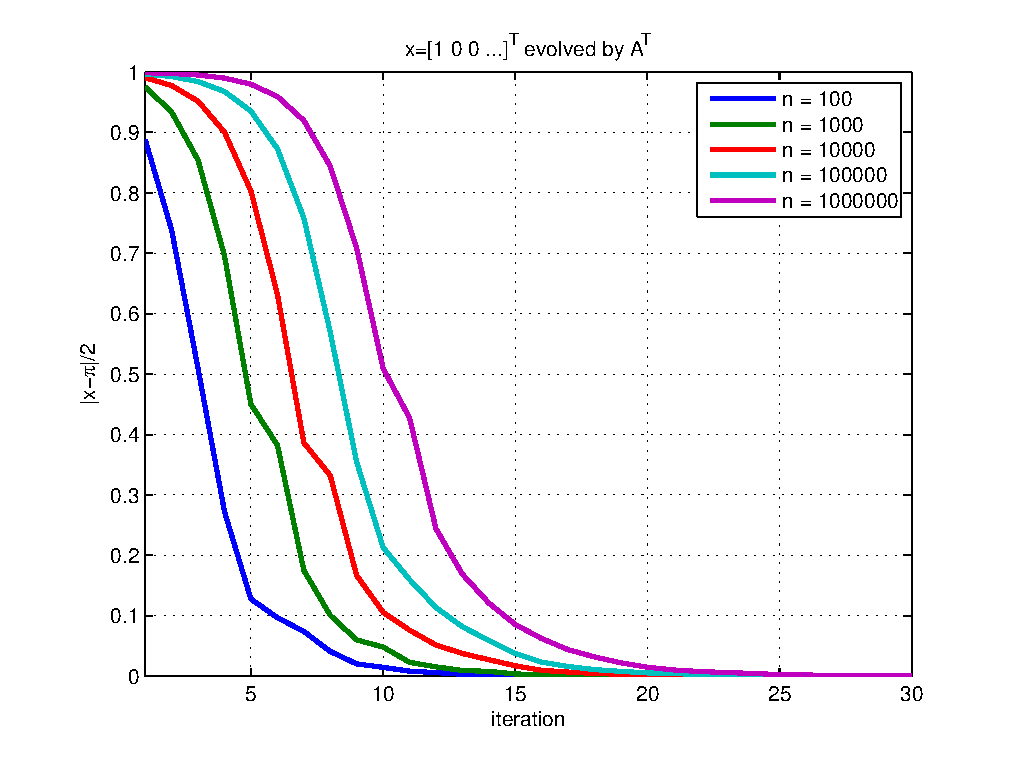
\includegraphics[width=0.44\textwidth,trim=1cm 1cm 0cm 0cm]{logisticxcutoff}&
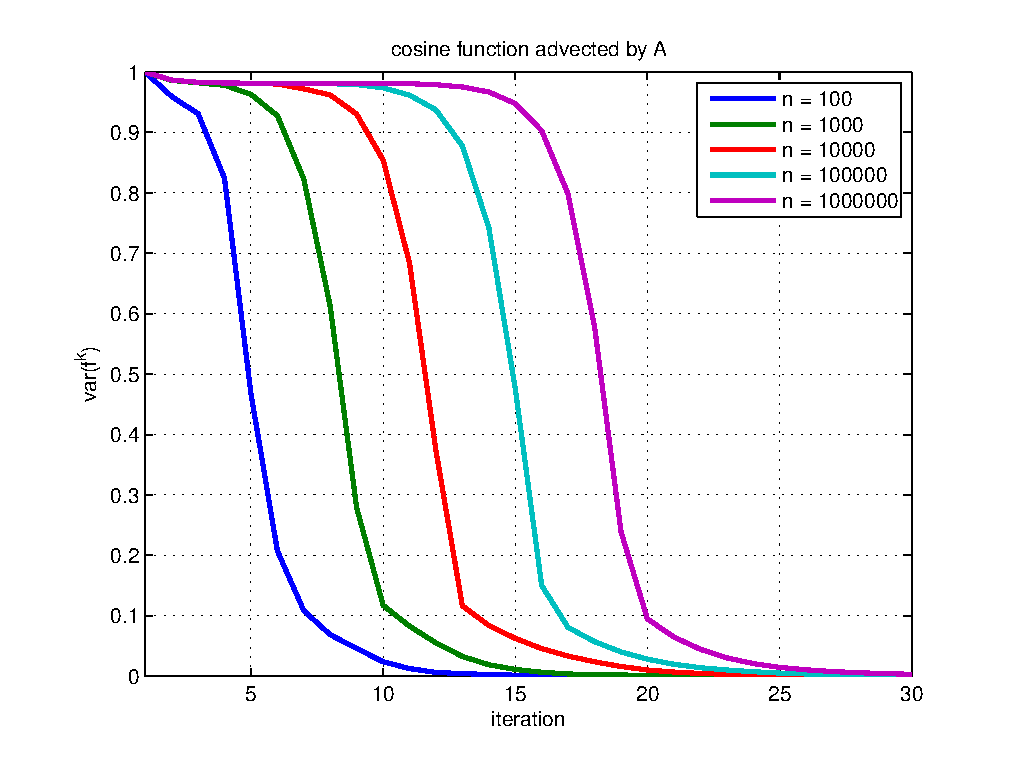
\includegraphics[width=0.44\textwidth,trim=1cm 1cm 0cm 0cm]{logisticfcutoff}
\end{tabular}

Left: $\omega^{k+1} = A^T \omega^{k}$

Right: $f^{k-1} = A f^{k}$
%%%%%%%%%%%%%%%%%%%%%%%%%%%%%%%%%%%%%%%%%%%%%%%%%%%%%%%%%%%%%%%%%%%%%%%%%%
\newpage
\oursection{A Lower bound of the Process}
In each row of $A$, there are at most $w$($w=4$ in logistic map) nonzeros. At $k$-th iteration, there are at most $w^k$ number of states are nonzeros. This gives us an lower bound on total variation diatance.
\begin{eqnarray*}
||x^k-\pi||_{TV} \ge 1-\frac{4}{\pi}\sin^{-1}\sqrt{\frac{w^k}{2n}} \mbox{   , when } w^k \le 2n
\end{eqnarray*}
Note the sequence of lower bounds indexed by $n$ presents a cutoff. 



%%%%%%%%%%%%%%%%%%%%%%%%%%%%%%%%%%%%%%%%%%%%%%%%%%%%%%%%%%%%%%%%%%%%%%%%%%
\newpage
\begin{tabular}{rl}%\setlength{\tabcolsep}{-30mm}
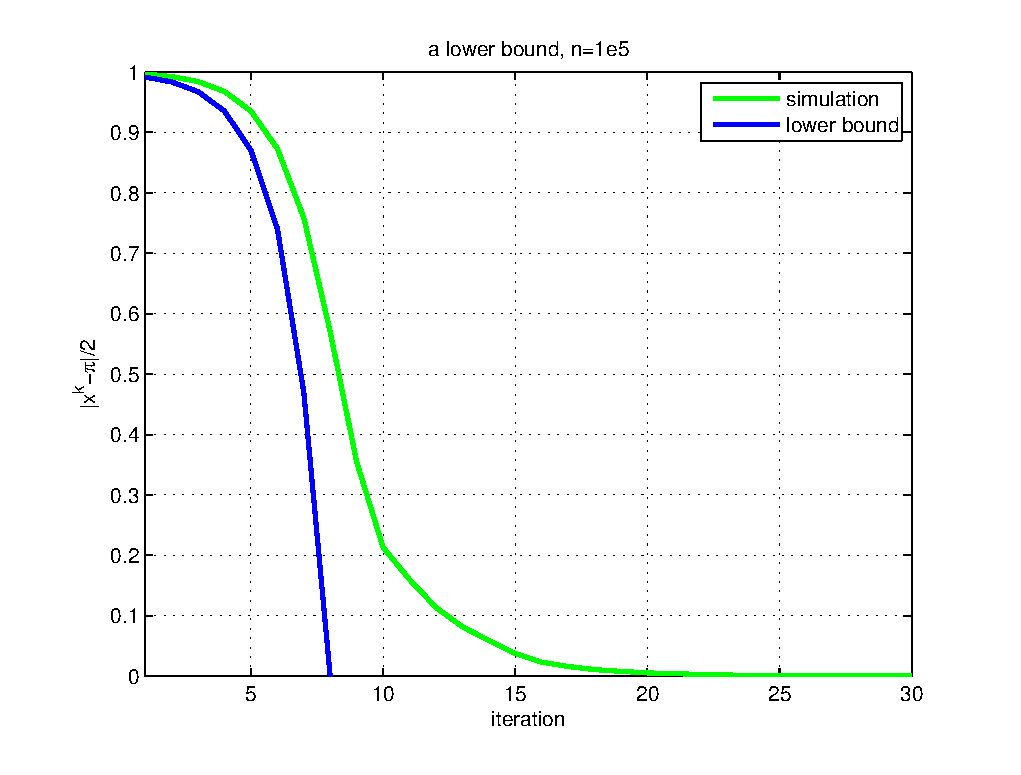
\includegraphics[width=0.45\textwidth,trim=1cm 1cm 0cm 0cm]{logisticlowerbound}
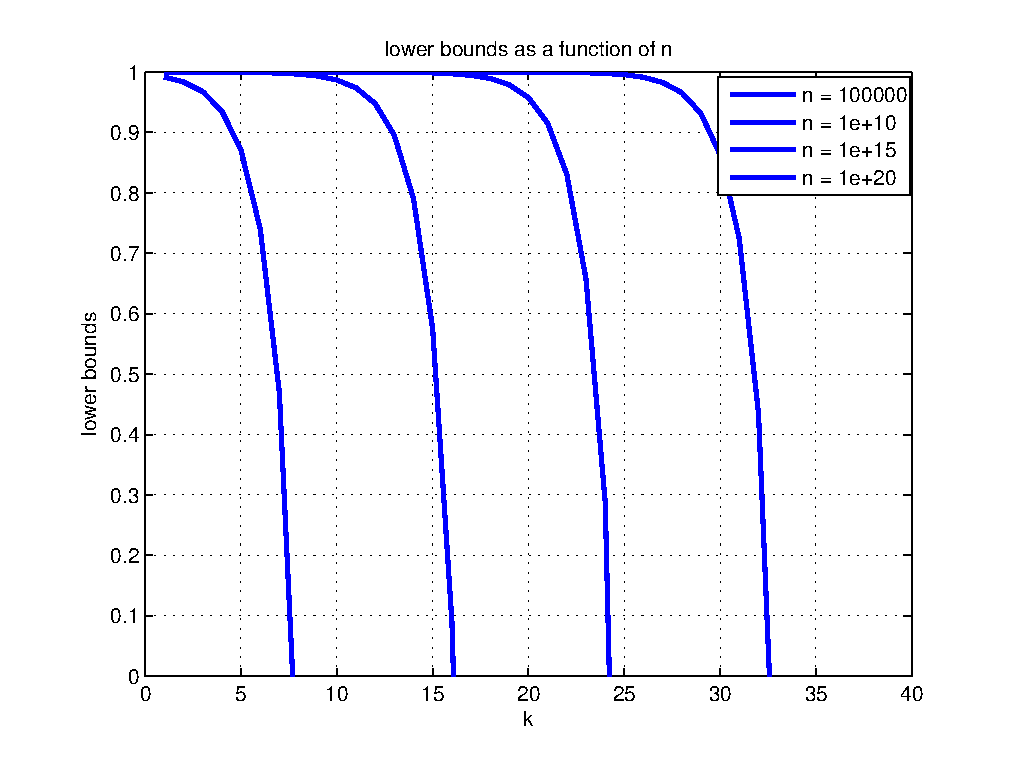
\includegraphics[width=0.45\textwidth,trim=1cm 1cm 0cm 0cm]{asinlowerbound}
\end{tabular}


Left: One example of the lower bound versus the simulation trajectory. 

Right: The sequence of lower bounds presents a cutoff.
%%%%%%%%%%%%%%%%%%%%%%%%%%%%%%%%%%%%%%%%%%%%%%%%%%%%%%%%%%%%%%%%%%%%%%%%%%
\newpage
\centerline{
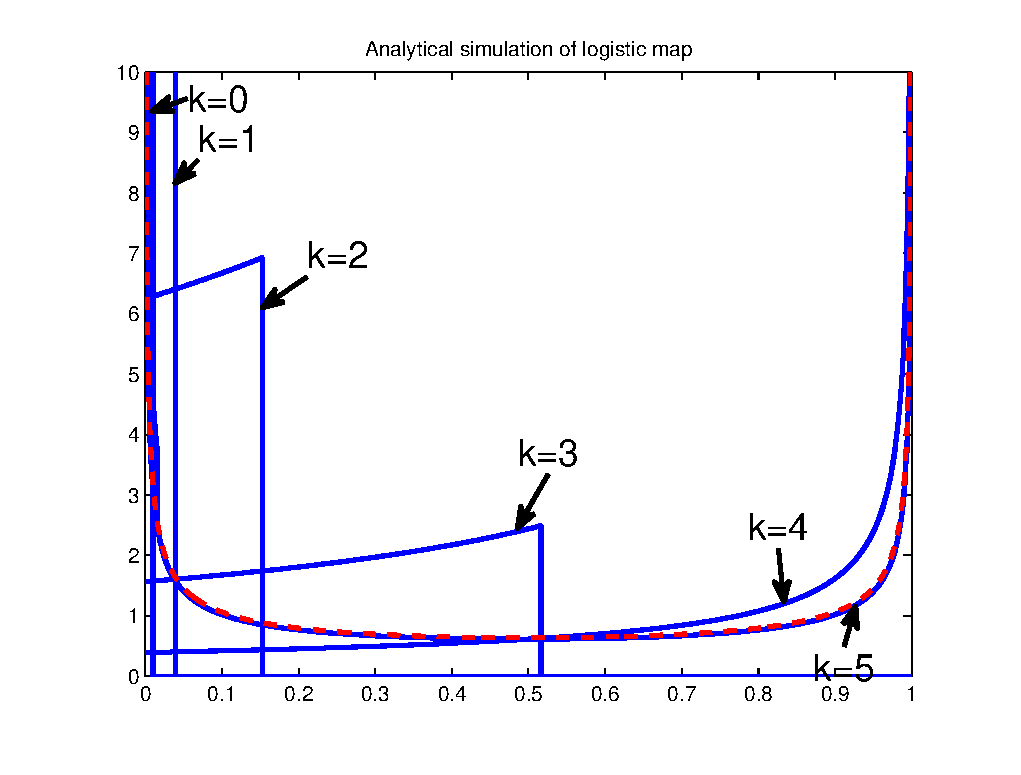
\includegraphics[width=0.42\textwidth,trim=1cm 1cm 0cm 0cm]{logisticmapanalyticalsimulation}
}
\begin{eqnarray*}
\omega^0 = \left\{\begin{tabular}{c}
           100, \mbox{ if} $x \le\frac{1}{100}$,\\ 
           0, \mbox{ otherwise}
           \end{tabular}\right.
\end{eqnarray*}
Dashed line is $\omega = \frac{1}{\pi\sqrt{x(1-x)}} $, the invariant distribution of logistic map. At the $5$-th iteration, is is almost invariant! 
%%%%%%%%%%%%%%%%%%%%%%%%%%%%%%%%%%%%%%%%%%%%%%%%%%%%%%%%%%%%%%%%%%%%%%%%%%
\newpage
\oursection{Conclusion}
\begin{itemize}
\item
The above simulation is done analytically. It shows that once the distribution is nonvanishing everywhere, the invariant distribution is almost achieved. This might be useful to prove the upper bound after cutoff. 
\end{itemize}





\end{document}


















